\documentclass[fleqn,11pt]{report}
\usepackage{amsmath,amssymb,esint}
\usepackage{amsthm,fixmath}
\usepackage[english]{babel}
\usepackage[a4paper,total={170mm,257mm},]{geometry}
\usepackage{epsfig}
\usepackage[format=hang,justification=centering]{subfig}
\usepackage{multirow}
\usepackage[square,comma,numbers,sort&compress]{natbib}
\usepackage{graphics}
\usepackage{graphicx}
\usepackage{hyperref}
\usepackage{float}
\usepackage{enumitem}
\usepackage{color}
\usepackage[x11names]{xcolor}
\usepackage{setspace}
\usepackage{listings}
\usepackage[UKenglish]{isodate}
\usepackage{fancybox}
\usepackage{fancyheadings,tabularx}
\usepackage{longtable}
\usepackage{ulem}

\pagestyle{fancyplain}  

\definecolor{C_Green}{rgb}{0,0.6,0}
\definecolor{C_Gray}{rgb}{0.5,0.5,0.5}
\definecolor{G_Purple}{rgb}{0.58,0,0.82}
\definecolor{C_Background}{rgb}{0.95,0.95,0.92}

\lstdefinestyle{CStyle}{
    backgroundcolor=\color{C_Background},   
    commentstyle=\ttfamily\color{C_Green},
    keywordstyle=\ttfamily\color{magenta},
    numberstyle=\ttfamily\tiny\color{C_Gray},
    stringstyle=\ttfamily\color{G_Purple},
    basicstyle=\ttfamily\footnotesize,
    breakatwhitespace=false,         
    breaklines=true,                 
    captionpos=b,                    
    keepspaces=true,                 
    numbers=left,                    
    numbersep=5pt,                  
    showspaces=false,                
    showstringspaces=false,
    showtabs=false,                  
    tabsize=2,
    language=C
}

\graphicspath{{figures/}} 

\usepackage[intoc]{nomencl}
\setcounter{secnumdepth}{3}
\setcounter{tocdepth}{2}
\setcounter{topnumber}{4}
\setcounter{totalnumber}{5}
\renewcommand{\topfraction}{1}
\renewcommand{\bottomfraction}{1}
\renewcommand{\textfraction}{0.01}
\newfloat{Program}{h}{lop}[chapter]
\newcommand{\HRule}{\rule{\linewidth}{0.5mm}}
\newcommand{\thedate}{\today}
\cleanlookdateon

\pagestyle{fancy}
\renewcommand{\headrulewidth}{0pt}
\renewcommand{\footrulewidth}{0.4pt}
\fancyhf{}
\lfoot{https://github.com/polycfd/apecss}
\cfoot{\thepage}
\rfoot{\thedate}

\fancypagestyle{plain}{%
  \fancyhf{}%
  \lfoot{https://github.com/polycfd/apecss}
  \cfoot{\thepage}
  \rfoot{\thedate}
  \renewcommand{\headrulewidth}{0pt}% Line at the header invisible
  \renewcommand{\footrulewidth}{0.4pt}% Line at the footer visible
}

\hypersetup{colorlinks = true, urlcolor = RoyalBlue3, linkcolor = RoyalBlue3, citecolor = RoyalBlue3}

\setlength{\parindent}{0cm}
\setlength{\parskip}{0.7em}
\setlength{\itemsep}{1pt}
\renewcommand{\em}{\it}
%%%%%%%%%%%%%%%%%%%%%%%%%%%%%%%%%%%%%%%%%%%%%%%%%%%%%%%%%%%%%%%%
\begin{document}
% Title Page
\begin{titlepage}
\begin{center}
% Upper part of the page
\null \vfill
% Title
\HRule \\[0.4cm]
{\huge APECSS}\\[0.05cm] {\large (Acoustic Pulse Emitted by Cavitation in Spherical Symmetry)}\\[0.1cm]
\HRule \\[2cm]

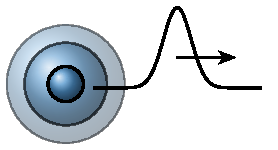
\includegraphics[width=7cm]{figures/apecssbubble.pdf}

\vspace{5cm}
Fabian Denner\\
S\"oren Schenke
\vfill

\thedate

\end{center}
\end{titlepage}

{\hypersetup{linkcolor=black}
\tableofcontents 
}

\chapter{About APECSS}

APECSS is a software tool to compute pressure-driven bubble dynamics and the resulting acoustic emissions. It is written exclusively in C and has been developed with simplicity, versatility and performance in mind. The acronym APECSS stands for "Acoustic Pulse Emitted by Cavitation in Spherical Symmetry".

The main features of APECSS are:\vspace{-1em}
\begin{itemize}[noitemsep]
\item Includes widely-used models for the bubble dynamics (Rayleigh-Plesset, Keller-Miksis, Gilmore).
\item Acoustic emissions of the bubble under different assumptions (incompressible, quasi-acoustic, fully compressible).
\item Prediction of the formation and attenuation of shock fronts emitted by the bubble.
\item Viscoelastic media (Kelvin-Voigt, Zener, Oldroyd-B).
\item Lipid monolayer coating of the bubble as used for ultrasound contrast agents.
\item All ODEs are solved with an in-built fifth-order Runge-Kutta scheme with fourth-order error estimate, based on \citet{Dormand1980}.
\item APECSS has no external dependencies, aside from some common C headers (math.h, stdio.h, stdlib.h, string.h).
\end{itemize}

The APECSS repository is located at \href{https://github.com/polycfd/apecss}{\texttt{https://github.com/polycfd/apecss}} and structured as follows:\vspace{-1em}
\begin{itemize}[noitemsep]
    \item The {\tt documentation/} folder contains a short documentation of APECSS, written in Latex.
    \item The {\tt examples/} folder contains representative examples of how to use APECSS and to demonstrate the most important features of APECSS. These examples also serve to validate APECSS against results reported in the literature.
    \item The {\tt include/} folder contains the {\tt apecss.h} header file, in which all variable, macro and function of APECSS are defined.
    \item The {\tt lib/} folder in which the APECSS library is compiled (at least if you follow the \ref{sec:installation}).
    \item The {\tt src} folder contains all source files ({\tt *.c}) of APECSS.
    \item The {\tt .clang-format} file, which defines the formatting rules for the source code. A \textit{clang} formatter (supported by most IDEs and editors) should be used for contributions to APECSS. The formatter should recognize this {\tt .clang-format} file automatically.
    \item The {\tt .gitignore} file telling \textit{git} which folders and files to ignore.
    \item The {\tt LICENSE.txt} file containing the Mozilla Public License Version 2.0.
    \item The {\tt README.txt} file with the most important information about APECSS.
\end{itemize}

APECSS is under the copyright of its developers and made available as open-source software under the terms of the \href{https://www.mozilla.org/en-US/MPL/2.0/}{Mozilla Public License Version 2.0}.

The development of APECSS has directly benefitted from research funding provided by the Deutsche Forschungsgemeinschaft (DFG, German Research Foundation), grant number 441063377.

\chapter{Using APECSS}

\section{Installation}
\label{sec:installation}

Installing APECSS is easy. After downloading APECSS in the folder {\tt <path to APECSS>}, define the following environment variables:\vspace{-1em}
\begin{itemize}[noitemsep]
\item {\tt APECSS\_DIR} to the folder in which APECSS is located. Using {\tt bash}, for instance, simply execute the command {\tt export APECSS\_DIR=<path to APECSS>} or, even better, add this command to your {\tt bash} profile.
\item {\tt USRLIB\_DIR} to the folder in which {\tt libm.a} or {\tt libm.dylib} (the standard \textit{math} library) is located. This may, for instance, be {\tt /usr/lib64/} on Linux systems or {\tt /usr/lib/} on MacOS systems.
\end{itemize}

Now, navigate into the folder {\tt \$APECSS\_DIR/lib} and execute {\tt ./compile\_lib.sh}. This shell script will compile the APECSS library using {\tt cmake} with the {\tt CMakeLists.txt} file provided in this folder. By default, APECSS is compiled with double precision and in \textit{Release} mode, meaning all optimization flags are enabled. That's it, you've successfully installed APECSS!

If you wish to install APECSS with \textit{Debug} flags, simply change the line
\begin{lstlisting}[style=CStyle,numbers=none]
  cmake CMakeLists.txt -DCMAKE_BUILD_TYPE=Release
\end{lstlisting}\vspace{-0.75em}
to
\begin{lstlisting}[style=CStyle,numbers=none]
  cmake CMakeLists.txt -DCMAKE_BUILD_TYPE=Debug
\end{lstlisting}\vspace{-0.75em}
in the {\tt ./compile\_lib.sh} shell script and, if applicable, in the shell script that compiles the desired example.

\section{Running APECSS}

There are several ways in which you can use the APECSS library. You can either incorporate selected features of APECSS into your own software code or you can program an interface to use APECSS as a standalone software tool. 

\subsection{The {\tt *.apecss} options file}

The {\tt *.apecss} file is the primary way of passing options, such as the size of the bubble, the density of the liquid or the type of results you want to have written out, to APECSS. 

Any {\tt *.apecss} file may contain the following sections (each terminated with {\tt END}):
\vspace{-1em}
\begin{itemize}[noitemsep]
  \item {\tt BUBBLE}: Information related to the bubble, such as its initial radius $R_0$ or the Rayleigh-Plesset model that is used to solve its dynamics.
  \item {\tt GAS}: Properties and equation of state of the gas.
  \item {\tt LIQUID}: Properties, type (i.e.~Newtonian or viscoelastic) and equation of state of the liquid.
  \item {\tt INTERFACE}: Properties of the gas-liquid interface. 
  \item {\tt RESULTS}: Results of the bubble dynamics and the acoustic emissions that should be written out.
  \item {\tt ODESOLVER}: Parameters of the ODE solver.
\end{itemize}
The options file is read by the functions {\tt apecss\_*\_readoptions()}. Any of the sections in the {\tt *.apecss} file, and any of the options that may be defined within each section, are optional; they are read if they are present, otherwise the default values (typically set in {\tt apecss\_*\_setdefaultoptions()}) or values set in the code calling it will be used. Comments can be added using {\tt \#}.

The relevant options that are available are discussed in the following chapters of this documentation in the context of the theoretical framework of APECSS. For instance, the available options used to define a certain Rayleigh-Plesset model are discussed in Section \ref{sec:rpmodels}, where the theory of the implemented Rayleigh-Plesset models is described. 

\subsection{Examples}

Some representative examples are available in the {\tt \$APECSS\_DIR/examples} folder. Each directory contains the following:\vspace{-1em}
\begin{itemize}[noitemsep]
  \item A {\tt README.md} file explaining the purpose and specificities of this/these example(s).
  \item A {\tt src/} folder with a file called {\tt *\_apecss.c} that acts as the standalone interface to the APECSS library. This file contains the {\tt main()} function and any additional functionality required to simulate a specific scenario.
  \item A {\tt build/} folder containing the {\tt CMakeLists.txt} file and a shell script {\tt compile.sh} with which this example can be compiled using the command {\tt ./compile.sh}.
  \item One or several {\tt *.apecss} file(s) in which the options for a specific case are defined.
\end{itemize}

In the examples provided in the {\tt \$APECSS\_DIR/examples} folder, the name of the  {\tt *.apecss} file is passed as an argument with the call to run APECSS, e.g.~executing {\tt ./<APECSS-example> -options run.apecss} to use an options file named {\tt run.apecss}.

Detailed information about each example, how to run it and what the results might be compared to can be found in the accompanying {\tt README.md} file.

\section{Programming in and with APECSS}

All functions are located in source files ({\tt *.c}) that relate to parts of the code, distinguished by physical phenomena (e.g.~{\tt emissions.c}), fluid type (e.g.~{\tt liquid.c}) or computational operations (e.g.~{\tt results.c}). 

All declarations and definitions are located in the header file {\tt include/apecss.h}. 

\subsection{Macros}

Macros are used as shortcuts to define frequently-used constants (e.g.~{\tt APECSS\_PI}), for frequently-used computational operations (e.g.~{\tt APECSS\_MAX}) and for computational operations that depend on the chosen machine precision (e.g.~{\tt APECSS\_SQRT}). Furthermore, options related to different numerical models are represented by logically named flags.

\subsubsection{Macros related to machine precision}

APECSS can be used with different floating point precisions: double precision (default) and long double precision ({\tt APECSS\_PRECISION\_LONGDOUBLE}).

Based on the chosen precision, {\tt APECSS\_FLOAT} is defined as the standard floating point type. In addition, the following precision-dependent computational operations are defined based on the chosen floating point precision:\vspace{-1em}
\begin{itemize}[noitemsep]
  \item {\tt APECSS\_ABS(a)}: Absolute value of $a$.
  \item {\tt APECSS\_CEIL(a)}: $a$ rounded to the nearest integer larger than $a$.
  \item {\tt APECSS\_COS(a)}: Cosine of $a$.
  \item {\tt APECCS\_EPS}: Returns a value that is close to machine epsilon.
  \item {\tt APECSS\_EXP(a)}: $\text{e}$ to the power $a$.
  \item {\tt APECSS\_LOG(a)}: Natural logarithm of $a$.
  \item {\tt APECSS\_POW(a,b)}: $a$ to the power $b$.
  \item {\tt APECSS\_SIN(a)}: Sine of $a$.
  \item {\tt APECSS\_SMALL}: Returns a number significantly smaller than machine epsilon.
  \item {\tt APECSS\_SQRT(a)}: Square root of $a$.
  \item {\tt APECSS\_STRINGTOFLOAT(a)}: Conversion of string $a$ to a float.
\end{itemize}
To ensure compatibility for different floating point precisions, it is paramount to use the standard floating point type {\tt APECSS\_FLOAT} and the operator definitions given above consistently throughout APECSS.

\subsubsection{Computational operations and predefined constants}

Macros that provide a shortcut to frequently-used computational operations are:\vspace{-1em}
\begin{itemize}[noitemsep]
  \item {\tt APECSS\_POW2(a)}: Returns $a^2$.
  \item {\tt APECSS\_POW3(a)}: Returns $a^3$.
  \item {\tt APECSS\_POW4(a)}: Returns $a^4$.
  \item {\tt APECCS\_MAX(a,b)}: Returns the maximum of $a$ and $b$.
  \item {\tt APECSS\_MAX3(a,b,c)}: Returns the maximum of $a$, $b$ and $c$.
  \item {\tt APECSS\_MIN(a,b)}: Returns the minimum of $a$ and $b$.
  \item {\tt APECSS\_MIN3(a,b,c)}: Returns the minimum of $a$, $b$ and $c$.
\end{itemize}

Macros that provide a shortcut to frequently-used constants are:\vspace{-1em}
\begin{itemize}[noitemsep]
  \item {\tt APECSS\_PI}: Returns $\pi=3.1415926535897932384626433832795028841972$.
  \item {\tt APECSS\_E}: Returns $\mathrm{e}=2.7182818284590452353602874713526624977572$.
  \item {\tt APECSS\_ONETHIRD}: Returns $1/3$.
  \item {\tt APECSS\_ONESIXTH}: Returns $1/6$.
  \item {\tt APECCS\_AVOGADRO}: Returns the Avogadro constant, $N_\mathrm{A}=6.02214076 \times 10^{23} \, \mathrm{mol}^{-1}$.
  \item {\tt APECSS\_LN\_OF\_2}: Returns the natural logarithm of 2, $\ln(2)=0.693147180559945309$.
  \item {\tt APECSS\_LN\_OF\_10}: Returns the natural logarithm of 10, $\ln(10)=2.302585092994045684$.
  \item {\tt APECSS\_LARGE}: Returns a large number, defined as $10^{15}$.
\end{itemize}

\subsubsection{Flags for model options}

All model options are represented by human-readable flags. 

If explicitly indicated as such, these flags are defined in such a way (with integer values being a multiple of 2), that a bit-wise comparison can be performed. Bit-wise comparison may be used for options that are checked frequently and for options that can have several building blocks.

Options of the embedded Runge-Kutta scheme of \citet{Dormand1980} used to discretize the governing ODEs:\vspace{-1em}
\begin{itemize}[noitemsep]
  \item {\tt APECSS\_RK54\_7M}: RK5(4)7M (minimum truncation) coefficients of \citet{Dormand1980}
  \item {\tt APECSS\_RK54\_7S}: RK5(4)7S (stability optimized) coefficients of \citet{Dormand1980}
\end{itemize}

Rayleigh-Plesset schemes:\vspace{-1em}
\begin{itemize}[noitemsep]
  \item {\tt APECSS\_BUBBLEMODEL\_RP}: Standard Rayleigh-Plesset model, Eq.~\eqref{eq:standardRP}.
  \item {\tt APECSS\_BUBBLEMODEL\_RP\_ACOUSTICRADIATION}: Rayleigh-Plesset model with acoustic radiation damping, Eq.~\eqref{eq:modRP}.
  \item {\tt APECSS\_BUBBLEMODEL\_KELLERMIKSIS}: Keller-Miksis model, Eq.~\eqref{eq:keller}.
  \item {\tt APECSS\_BUBBLEMODEL\_GILMORE}: Gilmore model, Eq.~\eqref{eq:gilmore}.
\end{itemize}

Equation of state of the gas:\vspace{-1em}
\begin{itemize}[noitemsep]
  \item {\tt APECSS\_GAS\_IG}: Ideal gas EoS.
  \item {\tt APECSS\_GAS\_HC}: Ideal gas EoS with van-der-Waals hardcore.
  \item {\tt APECSS\_GAS\_NASG}: Noble-Abel-stiffened-gas EoS.
\end{itemize}

Equation of state of the liquid:\vspace{-1em}
\begin{itemize}[noitemsep]
  \item {\tt APECSS\_LIQUID\_TAIT}: Tait EoS.
  \item {\tt APECSS\_LIQUID\_NASG}: Noble-Abel-stiffened-gas EoS.
\end{itemize}

Viscoelasticity of the liquid:\vspace{-1em}
\begin{itemize}[noitemsep]
  \item {\tt APECSS\_LIQUID\_NEWTONIAN}: Newtonian liquid.
  \item {\tt APECSS\_LIQUID\_KELVINVOIGT}: Kelvin-Voigt solid.
  \item {\tt APECSS\_LIQUID\_ZENER}: Zener solid (standard linear solid model).
  \item {\tt APECSS\_LIQUID\_OLDROYDB}: Oldroyd-B liquid.
\end{itemize}

Lipid monolayer coating of the gas-liquid interface (bit-wise):\vspace{-1em}
\begin{itemize}[noitemsep]
  \item {\tt APECSS\_LIPIDCOATING\_NONE}: No lipid monolayer coating.
  \item {\tt APECSS\_LIPIDCOATING\_MARMOTTANT}: Lipid monolayer coating described by the model of \citet{Marmottant2005}.
  \item {\tt APECSS\_LIPIDCOATING\_GOMPERTZFUNCTION}: Redefine the Marmottant model with a Gompertz function \citep{Guemmer2021}.
\end{itemize}

Acoustic excitation applied to the bubble:\vspace{-1em}
\begin{itemize}[noitemsep]
  \item {\tt APECSS\_EXCITATION\_NONE}: No external excitation. 
  \item {\tt APECSS\_EXCITATION\_SIN}: Sinusoidal excitation.
\end{itemize}

Model to compute the acoustic emissions of the bubble (bit-wise):\vspace{-1em}
\begin{itemize}[noitemsep]
  \item {\tt APECSS\_EMISSION\_NONE}: Emissions are not modelled.
  \item {\tt APECSS\_EMISSION\_INCOMPRESSIBLE}: Emissions are assumed to occur in an incompressible fluid.
  \item {\tt APECSS\_EMISSION\_FINITE\_SPEED\_INCOMPRESSIBLE}: Emissions are assumed to occur in an incompressible fluid, but the finite propagation speed given by the speed of sound is taken into account.
  \item {\tt APECSS\_EMISSION\_QUASIACOUSTIC}: Emissions are modelled under the quasi-acoustic assumption of \citet{Trilling1952} and \citet{Gilmore1952}.
  \item {\tt APECSS\_EMISSION\_KIRKWOODBETHE}: A model based on the Kirkwood-Bethe hypothesis (EKB, GFC, HPE) is used.
  \item {\tt APECSS\_EMISSION\_EV}: Emissions are modelled using the explicit expression based on the Kirkwood-Bethe hypothesis.
  \item {\tt APECSS\_EMISSION\_SIV}: Emissions are modelled using the spatially-integrated velocity, based on the Kirkwood-Bethe hypothesis, of \citet{Gilmore1952}.
  \item {\tt APECSS\_EMISSION\_TIV}: Emissions are modelled using the temporally-integrated velocity, based on the Kirkwood-Bethe hypothesis, of \citet{Hickling1963}.
\end{itemize}

\subsubsection{Others}
\label{sec:using_macros_others}

Macros for the output of certain results produced by APECSS:\vspace{-1em}
\begin{itemize}[noitemsep]
  \item {\tt APECSS\_RESULTS\_DISCARD}: Discard the results and do not write results to file.
  \item {\tt APECSS\_RESULTS\_WRITE}:  Write all data to file in one go.
  \item {\tt APECSS\_RESULTS\_APPEND}: Append the results file with a new batch of results.
\end{itemize}

Other predefined macros are used to define the length of strings and arrays, as well as to help with debugging:\vspace{-1em}
\begin{itemize}[noitemsep]
  \item {\tt APECSS\_DATA\_ALLOC\_INCREMENT}: The increment for dynamic re-allocation of arrays.
  \item {\tt APECSS\_STRINGLENGTH}: The standard length of a string.
  \item {\tt APECSS\_STRINGLENGTH\_SPRINTF}: The standard length of a string to be written out in the terminal.
  \item {\tt APECSS\_STRINGLENGTH\_SPRINTF\_LONG}: The standard length of a long string to be  written out in the terminal.
  \item {\tt APECSS\_WHERE}: Outputs in the terminal the file name and line number where the macro is called.
  \item {\tt APECSS\_WHERE\_INT(a)}: Outputs in the terminal the file name and line number where the macro is called, plus the integer value $a$.
  \item {\tt APECSS\_WHERE\_FLOAT(a)}: Outputs in the terminal the file name and line number where the macro is called, plus the floating point value $a$.
\end{itemize}


\subsection{Structures}

Structures ({\tt struct}) are used in APECSS to group variables and functions, and to provide a modular layout of the code that enables reusing different parts of it.

The structure {\tt APECSS\_Bubble} is the central structure of APECSS as it contains all the information related to a bubble. There is, of course, no {\it a priori} limit on how many copies of this structure a simulation can have, for instance, a multi-bubble simulation with 100 bubbles would naturally have 100 objects of type {\tt struct APECSS\_Bubble}. Aside from key information about the bubble, such as the bubble radius, the {\tt APECSS\_Bubble} structure contains pointers to the properties of the liquid the bubble is immersed in ({\tt struct APECSS\_Liquid}), the properties of the gas the bubble contains ({\tt struct APECSS\_Gas}) as wel as the properties of its interface ({\tt struct APECSS\_Interface}). If applicable, the {\tt APECSS\_Bubble} structure also points to the structure with the information of the driving acoustic excitation ({\tt struct APECSS\_Excitation}), the structure handling the acoustic emissions ({\tt struct APECSS\_Emissions}), and the structure containing the desired results ({\tt struct APECSS\_Results}). 

The (optional) structure {\tt APECSS\_Emissions} is, as the name suggests, related to the acoustic emissions of a bubble. If allocated, it contains information about how to handle the acoustic emissions, function pointers referring to the functions used to advance the acoustic emissions using a Lagrangian wave tracking approach and, very importantly, the linked list of emissions nodes ({\tt struct APECSS\_EmissionNode}) that carry the actual information of the acoustic emissions. The structure {\tt APECSS\_EmissionNode}  holds the information (e.g.~radial position, velocity, enthalpy, pressure) associated with a specific emission node.

The (optional) structure {\tt APECSS\_Results} holds all the results the user may want to have written out. For performance reasons, the results are in general not written to disk on-the-fly, but are stored in arrays and dumped to disk at the end of the simulation. The {\tt APECSS\_Results} structure contains optional structures for the results of the Rayleigh-Plesset model ({\tt struct APECSS\_ResultsBubble}) and for the acoustic emissions ({\tt APECSS\_ResultsEmissions}).

\subsection{Important functions}

Whenever using APECSS, at least one {\tt APECSS\_Bubble} structure has to be available and, if multiple bubbles are part of a simulation, each bubble has to be represented by a separate {\tt APECSS\_Bubble} structure. A single {\tt APECSS\_Bubble} structure is allocated and initialized as follows:
\begin{lstlisting}[style=CStyle,numbers=none]
  struct APECSS_Bubble *Bubble = (struct APECSS_Bubble *) malloc(sizeof(struct APECSS_Bubble));
  apecss_bubble_initializestruct(Bubble);
\end{lstlisting}\vspace{-0.75em}
The function {\tt apecss\_bubble\_initializestruct()} ensures that all pointers (to arrays, other structures and functions) that are part of the {\tt APECSS\_Bubble} structure are initialized to {\tt NULL}. This is important because the processing of options and any checks for allocation depend on {\tt NULL} to indicate that a given pointer in not yet allocated or not in use.
Then, we wish to set default values for the bubble parameters and read the relevant options from the options file:
\begin{lstlisting}[style=CStyle,numbers=none]
  apecss_bubble_setdefaultoptions(Bubble);
  apecss_bubble_readoptions(Bubble, OptionsDir);
\end{lstlisting}\vspace{-0.75em}
While setting default values is strongly advised, it is optional. The relative path to the options file may be set as
\begin{lstlisting}[style=CStyle,numbers=none]
char OptionsDir[APECSS_STRINGLENGTH];
sprintf(OptionsDir, "./run.apecss"); // Relative path to the options file.
\end{lstlisting}

In general, the properties of a gas ({\tt struct APECSS\_Gas}), a liquid ({\tt struct APECSS\_Liquid}) and a gas-liquid interface ({\tt struct APECSS\_Interface}), as well as the parameters for the ODE solver ({\tt struct APECSS\_NumericsODE}), have to be associated with a bubble, through the structure pointers {\tt *Gas}, {\tt *Liquid}, {\tt *Interface} and {\tt *NumericsODE} readily available in the {\tt APECSS\_Bubble} structure. In a single-bubble simulation this is obviously straightforward, we have one gas, one liquid and one interface that are associated with the bubble. In addition we have one set of solver parameters. In a multi-bubble simulation, however, we likely also have, for instance, only a single liquid (i.e.~all bubbles are situated in the same body of liquid), to which, in this case, all bubbles are associated to. Generally, the user is free in defining as many gases, liquids, interfaces and sets of solver parameters as deemed necessary, the only rule is that each bubble has to be associated with a gas, a liquid, an interface and a single set of solver parameters. Once these structures holding the fluid properties and the solver parameters are allocated, default values ought to be set, the user-defined options are read from file and the bubble(s) is/are successfully associated with its/their desired fluid properties and solver parameters. For a single-bubble simulation, this may look in a general form like:
\begin{lstlisting}[style=CStyle,numbers=none]
  struct APECSS_Gas *Gas = (struct APECSS_Gas *) malloc(sizeof(struct APECSS_Gas));
  struct APECSS_Liquid *Liquid = (struct APECSS_Liquid *) malloc(sizeof(struct APECSS_Liquid));
  struct APECSS_Interface *Interface = (struct APECSS_Interface *) malloc(sizeof(struct APECSS_Interface));
  struct APECSS_NumericsODE *NumericsODE = (struct APECSS_NumericsODE *) malloc(sizeof(struct APECSS_NumericsODE));

  apecss_gas_setdefaultoptions(Gas);
  apecss_liquid_setdefaultoptions(Liquid);
  apecss_interface_setdefaultoptions(Interface);
  apecss_odesolver_setdefaultoptions(NumericsODE);

  apecss_gas_readoptions(Gas, OptionsDir);
  apecss_liquid_readoptions(Liquid, OptionsDir);
  apecss_interface_readoptions(Interface, OptionsDir);
  apecss_odesolver_readoptions(NumericsODE, OptionsDir);

  Bubble->Gas = Gas;
  Bubble->Liquid = Liquid;
  Bubble->Interface = Interface;
  Bubble->NumericsODE = NumericsODE;
\end{lstlisting}\vspace{-0.75em}
Note that opening and reading the options file from disk is a relatively expensive (we are talking about a few microseconds) operation. For some of the single-bubble examples in {\tt \$APECSS\_DIR/examples} reading the options file is the most expensive operation by some margin. Therefore, if performance is of the essence, it might be worth hard coding the options instead of reading the options file.

After reading the options file, the {\tt apecss\_*\_processoptions()} functions are called to process options and make the relevant modeling choices:
\begin{lstlisting}[style=CStyle,numbers=none]
  apecss_gas_processoptions(Gas);
  apecss_liquid_processoptions(Liquid);
  apecss_interface_processoptions(Interface);
  apecss_odesolver_processoptions(NumericsODE);
  apecss_bubble_processoptions(Bubble);
\end{lstlisting}\vspace{-0.75em}
Processing the given options \uline{correctly} is critical to the working of APECSS.

Now that all options have been read and processed, the bubble has to be initialized based on the given options. This includes, for instance, computing the initial gas pressure inside the bubble (if it is not specified by the user) or, if applicable, the hardcore radius of the bubble.
\begin{lstlisting}[style=CStyle,numbers=none]
  apecss_bubble_initialize(Bubble);
\end{lstlisting}

The heart of APECSS is, of course, the solver for the bubble dynamics. The solver is split into three separate functions that (i) initialize the solver, (ii) run the solver and (iii) wrap up (i.e.~finalize) the solver:
\begin{lstlisting}[style=CStyle,numbers=none]
  apecss_bubble_solver_initialize(Bubble);
  apecss_bubble_solver_run(tend, Bubble);
  apecss_bubble_solver_finalize(Bubble);
\end{lstlisting}\vspace{-0.75em}
The initialization of the solver with {\tt apecss\_bubble\_solver\_initialize()} makes sure all counters, the solution error variable and, if applicable, result variables are initialized correctly. The function {\tt apecss\_bubble\_solver\_run()} contains the time-stepping procedure that executes the solver until a specified end time {\tt tend}, given as the first argument of the function call. In the examples found in {\tt \$APECSS\_DIR/examples}, the function {\tt apecss\_bubble\_solver\_run()} is only called once with {\tt tend = Bubble->tEnd}, i.e.~the end of the simulation. However, the user is free to call the function {\tt apecss\_bubble\_solver\_run()} an \uline{arbitrary number of times}, with any meaningful end time. This facilitates coupling APECSS to other numerical software frameworks, where {\tt tend} then could for instance be the end of the next time-step of a fluid dynamics solver. As an example simply chopping the simulation up into five equal-sized parts would look like:
\begin{lstlisting}[style=CStyle,numbers=none]
  apecss_bubble_solver_initialize(Bubble);
  apecss_bubble_solver_run(0.2 * tend, Bubble);
  apecss_bubble_solver_run(0.4 * tend, Bubble);
  apecss_bubble_solver_run(0.6 * tend, Bubble);
  apecss_bubble_solver_run(0.8 * tend, Bubble);
  apecss_bubble_solver_run(tend, Bubble);
  apecss_bubble_solver_finalize(Bubble);
\end{lstlisting}\vspace{-0.75em}
A solver run is ended with the function {\tt apecss\_bubble\_solver\_finalize()} where, for instance, the arrays and linked list of the acoustic emissions are freed.

\subsection{Output}
By default, APECSS does \uline{not} write out any output, neither to the terminal nor to a file. 

Basic information about the version and compile options of APECSS can be written out in the terminal using the function {\tt apecss\_infoscreen()} and any user-defined message by passing the desired string to the function {\tt apecss\_writeonscreen()}, as demonstrated in many of the available examples.

Various simulation results associated with the bubble dynamics and the acoustic emissions can be written to file by passing the appropriate options to APECSS (see Sections \ref{sec:bubble_results} and \ref{sec:emissions_results} for more details). In the interest of performance (writing data to file is very expensive), the results are stored in arrays and only written to file when the appropriate {\tt apecss\_results\_*\_write()} function is called, at the end of the simulation or at any appropriate point during the simulation, as shown in the examples. Exporting the results associated with the radial bubble dynamics using the function {\tt apecss\_results\_rayleighplesset\_write()} and the recording of the acoustic emissions at predefined spatial locations using the function {\tt apecss\_results\_emissionsspace\_write()} additionally requires the user to tell APECSS how the data should be handled, using the macros described in Section \ref{sec:using_macros_others}. Either the appropriate file is appended ({\tt APECSS\_RESULTS\_APPEND}), which makes sense if the results should be written out multiple times during a simulation, or the data is written to file in one go ({\tt APECSS\_RESULTS\_WRITE}), which should be used if the results are written out once at the end of the simulation. In both cases, the file is created automatically if it does not exist yet. Alternatively, the option {\tt APECSS\_RESULTS\_DISCARD} deletes the results without writing them to file, which can be useful if the results are used to collect, for instance, some statistics during the simulations but should not be stored in a file.

\subsection{The void data pointer}

Additional data associated with a bubble, an emission node, a gas, a liquid or an interface might be needed for more complex simulations, for instance neighbor information when multiple bubbles interact with each other or the thermal conductivity and heat capacity of the gas inside the bubble when heat transfer is considered. In APECSS, to retain flexibility and avoid unnecessary overhead, the structures {\tt struct APECSS\_Bubble}, {\tt struct APECSS\_EmissionNode}, {\tt struct APECSS\_Gas}, {\tt struct APECSS\_Liquid} and {\tt struct APECSS\_Interface} contain a \texttt{void} pointer called \texttt{user\_data} specifically for the purpose of associating additional data with those structures. This void pointer is not associated with a specific data type, but rather points to some memory location, i.e.~a memory address. 

A typical use of this void pointer would be to generate a structure that contains all additional data and point the void pointer to the address of this structure. For instance, the void pointer of the bubble structure is used in such a way in the example {\tt \$APECSS\_DIR/examples/laserinducedcavitation}. The structure
\begin{lstlisting}[style=CStyle,numbers=none]
  struct LIC
  {
    APECSS_FLOAT tauL, Rnbd, Rnc1, Rnc2, tmax1, tmax2;
  };
\end{lstlisting}\vspace{-0.75em}
is allocated
\begin{lstlisting}[style=CStyle,numbers=none]
  struct LIC *lic_data = (struct LIC *) malloc(sizeof(struct LIC));
\end{lstlisting}\vspace{-0.75em}
and associated with the void pointer
\begin{lstlisting}[style=CStyle,numbers=none]
  Bubble->user_data = lic_data;
\end{lstlisting}\vspace{-0.75em}
The data stored in this structure can then be used or read by again assigning the correct data type
\begin{lstlisting}[style=CStyle,numbers=none]
  struct LIC *lic_data = Bubble->user_data;
\end{lstlisting}\vspace{-0.75em}
and used as
\begin{lstlisting}[style=CStyle,numbers=none]
  tmax = lic_data->tmax1;
\end{lstlisting}\vspace{-0.75em}
At the end of the simulation, when the data is no longer needed, the memory occupied by the structure is freed
\begin{lstlisting}[style=CStyle,numbers=none]
  free(lic_data);
\end{lstlisting}%\vspace{-0.75em}

The example {\tt \$APECSS\_DIR/examples/gastemperature} uses both the void pointers associated with the bubble and the gas.

\subsection{A word on function pointers}

APECSS uses function pointers extensively. Function pointers are an elegant means in {\tt C} to add complexity and functionality yet still retain a slim code, avoid redundant code and, if nothing else, avoid a large number of costly conditional statements. However, function pointers can quickly make a code unreadable and obfuscate what is actually happening, if they are used without care. In order to keep the use of function pointers in APECSS transparent, the adopted convention is that \uline{all} function pointers are set in {\tt apecss\_*\_processoptions()} functions, e.g.~{\tt apecss\_gas\_processoptions()}.

\subsection{Code formatting}
\label{sec:clang}

To ensure a consistent formatting, please use a \textit{clang} formatter that formats the file automatically upon saving. The file defining the formatting of the APECSS source code ({\tt .clang-format}) is part of the repository. A \textit{clang} formatter (supported by most IDEs and editors) should be used for contributions to APECSS. The formatter should recognize this {\tt .clang-format} file automatically.

\section{Units}

APECSS assumes SI units or any appropriate combination of SI units at all times, e.g.~when reading user-defined options, in all internal computations and when outputting data. To avoid any misunderstanding, the SI base units are the following:  time in seconds [s], length in meter [m], mass in kilogram [kg], temperature in Kelvin [K], electric current in Ampere [A], amount of substance in mole [mol], luminosity in candela [cd].

\section{Automated testing}

Github {\it workflows} are run automatically to test the functionality of APECSS everytime a change is {\it pushed} to the {\tt main} branch of APECSS or if a {\it pull request} is opened.
This includes a {\tt Build test} and a {\tt Run test}, the results of which are displayed in the rendered {\tt README.md} file of the Github repository.

The {\tt Build test} checks whether the APECSS library compiles correctly on Linux and MacOS operating systems. The {\tt Run test}, also conducted on both Linux and MacOS operating systems, is more comprehensive, in that it first compiles the APECSS library, then compiles and runs each example. Note that a successful {\tt Run test} does not imply correct results - the {\tt Run test} only tests the basic functionality of the code (e.g.~no segmentation faults), not the correctness of the results APECSS produces. 

\section{Citing APECSS}

If you use APECSS for your scientific work, please consider citing the paper introducing the theoretical foundation of APECSS,\vspace{-0.5em}
\begin{itemize}[leftmargin=*]
  \item[] F.~Denner and S.~Schenke, Modeling acoustic emissions and shock formation of cavitation bubbles. \textit{Physics of Fluids} 35 (2023), 012114. \href{https://doi.org/10.1063/5.0131930}{\texttt{https://doi.org/10.1063/5.0131930}} 
\end{itemize}\vspace{-0.5em}
as well as the version of APECSS you've used for your work, e.g.\vspace{-0.5em}
\begin{itemize}[leftmargin=*]
  \item[] F.~Denner and S.~Schenke, APECSS (v1.2), \textit{Zenodo} (2022). \\ \href{https://doi.org/10.5281/zenodo.7465050}{\texttt{https://doi.org/10.5281/zenodo.7465050}}
\end{itemize}\vspace{-0.5em}
All releases can be found on the \href{https://doi.org/10.5281/zenodo.7249297}{Zenodo page} of APECSS.



\chapter{Bubble dynamics}
\label{chap:bubble}
The dynamic behaviour of the bubble is modelled with a Rayleigh-Plesset-type (RP) model, assuming spherical symmetry. This requires to choose a suitable RP-type model (Section \ref{sec:rpmodels}) and define appropriate conditions for the gas  (Section \ref{sec:gas}), the liquid (Section \ref{sec:liquid}), the interface (Section \ref{sec:interface}), as well as at infinity (Section \ref{sec:infinity}). The results that APECSS can write out based on the RP model are explained in Section \ref{sec:bubble_results}.

APECSS solves all ordinary differential equations (ODEs) associated with the bubble dynamics sing the embedded RK5(4) scheme of \citet{Dormand1980}, whereby a fifth-order Runge-Kutta scheme is used to solve the ODEs and the corresponding fourth-order Runge-Kutta scheme is used to estimate the solution error. Based on this solution error, the time-step $\Delta t$ used to advance the solution of the ODEs is adapted. If the solution error of a newly computed solution in a time-step does not satisfy the error tolerance, the solution is rewound and recomputed with a smaller $\Delta t$ (cf. sub-iteration), adapted based on the solution error of the previous attempt. 

\vspace{0.8em}

\noindent
\begin{tabular}{p{0.12\textwidth} p{0.32\textwidth} p{0.45\textwidth}}
    \textbf{Section} &\textbf{Command} & \textbf{Description} 
\vspace{1mm} \\ \hline
{\tt BUBBLE} & {\tt InitialRadius <float>} & The initial radius $R_0$ of the bubble.\\ 
 & {\tt PressureAmbient <float>} & The ambient pressure $p_0$.\\ 
 & {\tt InitialGasPressure <float>} & The initial gas pressure $p_{\mathrm{G},0}$, if different from $p_0$ or the corresponding Laplace pressure.\\ 
{\tt ODESOLVER} & {\tt RK 7M} & Minimum truncation (7M) coefficients of the RK5(4) scheme of \citet{Dormand1980}. This is the default.\\ 
& {\tt RK 7S} & Stability optimized (7S) coefficients of the RK5(4) scheme of \citet{Dormand1980}.\\ 
& {\tt Tolerance <float>} & The desired solution tolerance.\\ 
& {\tt MinTimeStep <float>} & Minimum time-step $\Delta t$.\\ 
& {\tt MaxTimeStep <float>} & Maximum time-step $\Delta t$.\\ 
& {\tt MaxSubIterations <float>} & Maximum number of sub-iterations in a given time-step.\\ 
 \hline
\end{tabular} \vspace{1em}

\section{Rayleigh-Plesset models}
\label{sec:rpmodels}

APECSS offers four RP-type models to simulate pressure-driven bubble dynamics: the standard Rayleigh-Plesset model without and with acoustic radiation damping, the Keller-Miksis model and the Gilmore model.

\vspace{0.8em}

\noindent
\begin{tabular}{p{0.12\textwidth} p{0.32\textwidth} p{0.45\textwidth}}
    \textbf{Section} &\textbf{Command} & \textbf{Description} 
\vspace{1mm} \\ \hline
{\tt BUBBLE} & {\tt RPModel RP} & Standard Rayleigh-Plesset model, Eq.~\eqref{eq:standardRP}. This is the default.\\ 
 & {\tt RPModel RPAR} & Rayleigh-Plesset model including acoustic radiation damping, Eq.~\eqref{eq:modRP}.\\ 
 & {\tt RPModel KM} & Keller-Miksis model, Eq.~\eqref{eq:keller}.\\ 
 & {\tt RPModel Gilmore} & Gilmore model, Eq.~\eqref{eq:gilmore}.\\ 
 \hline
\end{tabular} \vspace{1em}

\noindent The standard Rayleigh-Plesset (RP) model is given as \citep{Lauterborn2010}
\begin{equation}
R \ddot{R} + \frac{3}{2} \dot{R}^2 = \frac{p_\text{L} - p_\infty}{\rho_{\ell,\mathrm{ref}}},
\label{eq:standardRP}
\end{equation}
where $R$ is the bubble radius, $p_\text{L}$ is the pressure of the liquid at the bubble wall, $p_\infty$ is the pressure of the liquid in the far field, $p_\text{G}$ is the pressure of the gas inside the bubble and $\rho_{\ell,\mathrm{ref}}$ is the {\it constant} density of the liquid.

To incorporate acoustic radiation in the liquid and the associated damping, the modified Rayleigh-Plesset model is given as \citep{Brenner2002}
\begin{equation}
R \ddot{R} + \frac{3}{2} \dot{R}^2 = \frac{p_\text{L} - p_\infty}{\rho_{\ell,\mathrm{ref}}} + \frac{R \, \dot{p}_\text{G}}{\rho_{\ell,\mathrm{ref}} \, c_{\ell,\mathrm{ref}}} ,
\label{eq:modRP}
\end{equation}
where $c_{\ell,\mathrm{ref}}$ is the \textit{constant} reference speed of sound of the liquid. The last term on the right-hand side accounts for acoustic radiation in the liquid.
This modified RP model is frequently used to simulate medical ultrasound applications \citep{Versluis2020} as well as sonoluminescence \citep{Brenner2002}.
It follows directly from the Keller-Miksis model, Eq.~(\ref{eq:keller}), which incorporates the compressibility of the liquid, by assuming the Mach number of the bubble wall is vanishingly small, $M_\ell = \dot{R}/c_{\ell,\mathrm{ref}} \simeq 1$. Eq.~(\ref{eq:modRP}) is, consequently, only valid for small Mach numbers $M_\ell \ll 1$ \citep{Neppiras1980, Prosperetti1986}.

The Keller-Miksis model \citep{Keller1980, Prosperetti1986}, which incorporates the compressibility of the liquid to first order, is given as
\begin{equation}
\left(1 - \frac{\dot{R}}{c_{\ell,\mathrm{ref}}}\right) R \ddot{R} + \frac{3}{2} \left(1 - \frac{\dot{R}}{3\, c_{\ell,\mathrm{ref}}}\right) \dot{R}^2 =  \left(1 + \frac{\dot{R}}{c_{\ell,\mathrm{ref}}}\right) \frac{p_\text{L} - p_\infty}{\rho_{\ell,\mathrm{ref}}} + R \, \frac{\dot{p}_\text{L} - \dot{p}_\infty}{\rho_{\ell,\mathrm{ref}} \, c_{\ell,\mathrm{ref}}} ,
\label{eq:keller}
\end{equation}
where $c_{\ell,\mathrm{ref}}$ is the speed of sound of the liquid. Both $\rho_{\ell,\mathrm{ref}}$ and $c_{\ell,\mathrm{ref}}$ are assumed to be constant, limiting the Keller-Miksis model to moderate liquid pressures ($p_\mathrm{L} \lesssim 10^8 \, \mathrm{Pa}$).

Based on the Kirkwood-Bethe hypothesis \citep{Kirkwood1942,Cole1948}, \citet{Gilmore1952} derived a second-order ordinary differential equation describing the radial dynamics of a bubble in a compressible liquid, %given as
\begin{equation}
  \left( 1 - \frac{\dot{R}}{c_\text{L}} \right) R \ddot{R} + \frac{3}{2} \left( 1 - \frac{\dot{R}}{3 c_\text{L}} \right) \dot{R}^2  = \left( 1 + \frac{\dot{R}}{c_\text{L}} \right) H + \left( 1- \frac{\dot{R}}{c_\text{L}} \right) \frac{R \dot{H}}{c_\text{L}}, \label{eq:gilmore}
\end{equation} 
where $c_\mathrm{L}$ is the speed of sound of the liquid at the bubble wall, $H = h_\text{L} - h_\infty$ is the enthalpy difference between the bubble wall and infinity, and $\dot{H} = \dot{h}_\text{L} - \dot{h}_\infty$ is the derivative of $H$. The enthalpy $h$ and the speed of sound $c$ are defined by an appropriate equation of state as a function of pressure, with $h_\text{L} = h(p_\text{L})$, $h_\infty = h(p_\infty)$ and $c_\text{L} = c(p_\text{L})$, as detailed in \ref{sec:liquid}.

\section{The gas}
\label{sec:gas}

In APECSS, every bubble contains a gas, which requires to select an appropriate equation of state and define meaningful properties.

\vspace{0.8em}

\noindent
\begin{tabular}{p{0.1\textwidth} p{0.36\textwidth} p{0.49\textwidth}}
    \textbf{Section} &\textbf{Command} & \textbf{Description} 
\vspace{1mm} \\ \hline
{\tt GAS} & {\tt EoS IG} & Ideal gas equation of state. This is the default.\\ 
& {\tt EoS HC} & Ideal gas equation of state with van-der-Waals hardcore.\\ 
& {\tt EoS NASG} & Noble-Abel-stiffened-gas equation of state.\\
& {\tt PolytropicExponent <float>} & Polytropic exponent $\Gamma_\text{g}$.\\
& {\tt ReferencePressure <float>} & Reference pressure $p_\text{g,ref}$.\\
& {\tt ReferenceDensity <float>} & Reference density $\rho_\text{g,ref}$.\\
& {\tt CoVolume <float>} & Co-volume $b_\text{g}$.\\
& {\tt TaitPressureConst <float>} & Pressure constant $B_\text{g}$.\\
& {\tt MolecularWeight <float>} & Molecular weight $\mathcal{M}_{\text{g}}$ of the gas.\\
& {\tt MolecularDiameter <float>} & Molecular kinematic diameter $\mathcal{D}_{\text{g}}$ of the gas.\\
{\tt BUBBLE} & {\tt HardcoreRadius <float>} & Hardcore radius $r_\text{hc}$.\\
 \hline
\end{tabular} \vspace{1em}


Using the ideal gas EoS, the pressure and its derivative are given as
\begin{align}
  p_\text{G} &= p_\text{G,ref} \left(\frac{R_0}{R}\right)^{3 \Gamma_\text{g}}\\
  \dot{p}_\text{G} &= -3 \, \frac{p_\text{G} \, \Gamma_\text{g} \, \dot{R}}{R},\\
\end{align}
including a van-der-Waals hardcore (HC) in the ideal gas model, the pressure and its derivative follow as
\begin{align}
  p_\text{G} &= p_\text{G,ref} \left(\frac{R_0^3-r_\text{hc}^3}{R^3-r_\text{hc}^3}\right)^{\Gamma_\text{g}}\\
  \dot{p}_\text{G} &= -3 \, \frac{p_\text{G} \, \Gamma_\text{g} \, R^2 \, \dot{R}}{R^3-r_\text{hc}^3},
\end{align}
and using the Noble-Abel-stiffened-gas (NASG) EoS, the pressure and its derivative are \citep{Denner2021}
\begin{align}
  p_\text{G} &= (p_\text{G,ref} + B_\text{g}) \left[\frac{\rho_\text{g} \, (1-b_\text{g} \, \rho_\text{g,ref})}{\rho_\text{g,ref} \, (1- b_\text{g} \, \rho_\text{G})} \right]^{\Gamma_\text{g}} - B_\text{g}\\
  \dot{p}_\text{G} &= \frac{\dot{\rho}_\text{G} \, \Gamma_\text{g} \left(p_\text{G} + B_\text{g} \right)}{\rho_\text{G} \left(1- b_\text{g} \, \rho_\text{G} \right)},
\end{align}
where $\Gamma_\mathrm{g}$ is the polytropic exponent, $r_\mathrm{hc}$ is the hardcore radius, $b_\mathrm{g}$ is the co-volume and $B_\mathrm{g}$ is a pressure constant.

Assuming mass conservation, the gas density and its derivative are given by 
\begin{align}
  \rho_\text{G} &= \rho_\text{g,ref} \left(\frac{R_0}{R}\right)^3 \label{eq:rhoG}\\
  \dot{\rho}_\text{G} &= -3 \, \rho_\text{G}\, \frac{\dot{R}}{R}. \label{eq:dot_rhoG}
\end{align}

The hardcore radius $r_\mathrm{hc}$ and the co-volume $b_\mathrm{g}$ are set by default to $-1$. If the {\tt HC} or {\tt NASG} model is chosen, the user has to pass values for the hardcore radius $r_\mathrm{hc}$ or the co-volume $b_\mathrm{g}$, respectively. Alternatively, the molecular weight $\mathcal{M}_{\text{g}}$ and the molecular kinematic diameter $\mathcal{D}_{\text{g}}$ of the gas may be defined instead of $r_\mathrm{hc}$ or $b_\mathrm{g}$; APECSS then computes the correct co-volume $b_\mathrm{g}$ or, based on the bubble size, hardcore radius $r_\mathrm{hc}$. Assuming the molecular weight $\mathcal{M}_{\text{g}}$, the bubble contains 
\begin{equation}
    N_\mathrm{G} = N_\mathrm{A} \, \frac{\rho_{\mathrm{G},0} V_0}{\mathcal{M}_{\text{g}}} 
\end{equation}
molecules, where $N_\mathrm{A}$ is the Avogadro constant (see macro {\tt APECSS\_AVOGADRO}), $\rho_{\mathrm{G},0}$ is the initial gas density and $V_0$ is the initial bubble volume. As per the molecular kinetic diameter $\mathcal{D}_{\text{g}}$ of the gas molecules, the volume of each molecule is
\begin{equation}
    V_\mathrm{mol} = \frac{\pi}{6} \, \mathcal{D}_{\text{g}}^3.
\end{equation}
The van-der-Waals hardcore radius is then readily defined as
\begin{equation}
    r_\mathrm{hc} = \sqrt[3]{\frac{3}{4 \pi} f_\mathrm{mol} \, V_\mathrm{mol} \, N_\mathrm{G}}
\end{equation}
and the co-volume of the gas is given as
\begin{equation}
    b_\mathrm{g} = f_\mathrm{mol} \, N_\mathrm{A} \, \frac{V_\mathrm{mol}}{\mathcal{M}_{\text{g}}}.
\end{equation}
The semi-empirical constant $f_\mathrm{mol}$ is based on the repulsive forces acting between the molecules \citep{Kontogeorgis2019}, and is typically taken to be $f_\mathrm{mol}=4$.


\section{The liquid}
\label{sec:liquid}

In the same way that every bubble contains a gas, in APECSS every bubble is surrounded by a liquid, which requires to select an appropriate equation of state and fluid type, as well as define meaningful properties.

\vspace{0.8em}

\noindent
\begin{tabular}{p{0.1\textwidth} p{0.35\textwidth} p{0.5\textwidth}}
    \textbf{Section} &\textbf{Command} & \textbf{Description} 
\vspace{1mm} \\ \hline
{\tt LIQUID} & {\tt EoS Tait} & The Tait EoS is applied to the liquid. Only relevant for the Gilmore model and acoustic emissions based on the Kirkwood-Bethe hypothesis.\\ 
& {\tt EoS NASG} & The Noble-Abel-stiffened-gas EoS is applied to the liquid. Only relevant for the Gilmore model and acoustic emissions based on the Kirkwood-Bethe hypothesis.\\ 
& {\tt LiquidType Newtonian} & Newtonian fluid. This is the default.\\ 
& {\tt LiquidType KelvinVoigt} & Kelvin-Voigt solid.\\ 
& {\tt LiquidType Zener} & Zener solid.\\ 
& {\tt LiquidType OldroydB} & Oldroyd-B (or upper-convected Maxwell) fluid.\\ 
& {\tt PolytropicExponent <float>} & Polytropic exponent $\Gamma_{\ell}$.\\
& {\tt ReferencePressure <float>} & Reference pressure $p_{\ell,\text{ref}}$.\\
& {\tt ReferenceDensity <float>} & Reference density $\rho_{\ell,\text{ref}}$.\\
& {\tt ReferenceSpeedofSound <float>} & Reference speed of sound $\rho_{\ell,\text{ref}}$.\\
& {\tt CoVolume <float>} & Co-volume $b_\ell$.\\
& {\tt TaitPressureConst <float>} & Pressure constant $B_\ell$.\\
& {\tt Viscosity <float>} & Newtonian viscosity $\mu_\ell$.\\
& {\tt PolymerViscosity <float>} & Polymer viscosity $\eta_\ell$ associated with viscoelasticity.\\
& {\tt ShearModulus <float>} & Shear modulus $G_\ell$ associated with viscoelasticity.\\
& {\tt RelaxationTime <float>} & Relaxation time $\lambda_\ell$ associated with viscoelasticity.\\
 \hline
\end{tabular} \vspace{1em}

The pressure at the bubble wall of a Newtonian liquid is given as
\begin{equation}
  p_\text{L} = p_\text{G} - \frac{2 \sigma}{R} - 4 \, \mu_\ell \frac{\dot{R}}{R}, \label{eq:pL}
\end{equation}
where $p_\text{G}$ is the gas pressure, see Section \ref{sec:gas}, $\sigma$ is the surface tension coefficient of the interface, see Section \ref{sec:interface}, and $\mu_\ell$ is the liquid (Newtonian) viscosity. The derivative of Eq.~\eqref{eq:pL} follows as
\begin{equation}
  \dot{p}_\mathrm{L} = \dot{p}_\mathrm{G} + \frac{2 \, \sigma \, \dot{R}}{R^2} + 4 \, \mu_\ell \left(\frac{\dot{R}^2}{R^2} - \frac{\ddot{R}}{R}\right).
  \label{eq:dotpL}
\end{equation}

\subsection{Equation of state}

For the Gilmore model \eqref{eq:gilmore} and the acoustic emissions based on the Kirkwood-Bethe hypothesis (see Section \ref{sec:emissionskb}), an equation of state (EoS) for the liquid has to be defined. Two EoS are currently available in APECSS: the Tait EoS and the NASG EoS. 

Since the seminal work of \citet{Gilmore1952}, the Tait EoS is traditionally used to describe the properties of the liquid in Eq.~\eqref{eq:gilmore}. The Tait EoS defines the density $\rho$, enthalpy $h$ and speed of sound $c$ as
\begin{align}
    \rho &= \rho_{\ell,\text{ref}} \left( \frac{p+B_\ell}{p_{\ell,\text{ref}}+B_\ell}\right)^{\frac{1}{\Gamma_\ell}} \label{eq:rho_Tait} \\
    h &= \frac{\Gamma_\ell}{\Gamma_\ell-1} \frac{p+B_\ell}{\rho} \label{eq:h_Tait} \\
    c &= \sqrt{(\Gamma_\ell -1) \, h}, \label{eq:c_Tait}
\end{align}
respectively, where $B_\ell$ is a pressure constant, $\Gamma_\ell$ is the polytropic exponent, $p_{\ell,\text{ref}}$ is the reference pressure and $\rho_{\ell,\text{ref}}$ is the reference density. For water, typical values are $\Gamma_\ell=7.15$, $B_\ell=3.046 \times 10^8 \, \text{Pa}$, $\rho_{\ell,\text{ref}} = 997 \, \mathrm{kg/m}^3$ and $p_{\ell,\text{ref}} = 10^5 \, \mathrm{Pa}$. 

Using the Noble-Abel stiffened-gas (NASG) EoS \citep{LeMetayer2016} instead of the Tait EoS, the fluid properties are defined as \citep{Denner2021}
 \begin{eqnarray}
    \rho &=& \frac{K_\ell \, (p+B_\ell)^{\frac{1}{\Gamma_\ell}}}{1+b_\ell \, K_\ell \,  (p+B_\ell)^{\frac{1}{\Gamma_\ell}}} \label{eq:rho_NASG}\\
      h &=& \frac{\Gamma_\ell}{\Gamma_\ell-1} \frac{p+B_\ell}{\rho} - \frac{\Gamma_\ell \, b_\ell}{\Gamma_\ell-1} \, (p+B_\ell) + b_\ell \, p \label{eq:h_NASG} \\
      c &=&\sqrt{\Gamma_\ell \, \frac{(p+B_\ell)}{\rho-b_\ell  \rho^2}},\label{eq:c_NASG}
    \end{eqnarray}
with $K_\ell = \rho_{\ell,\text{ref}}/[(p_{\ell,\text{ref}}+B_\ell)^{{1/\Gamma_\ell}} \ (1-b_\ell \rho_{\ell,\text{ref}})]$ describing a constant reference state, and where $b_\ell$ is the co-volume of the liquid molecules. The NASG EoS reduces to the Tait EoS for $b_\ell=0$. Appropriate properties for water have, for instance, been proposed by \citet{Chandran2019} as $\Gamma_\ell = 1.19$, $B_\ell = 6.2178 \times 10^{8} \, \mathrm{Pa}$, $b_\ell = 6.7212 \times 10^{-4} \, \mathrm{m}^3/\mathrm{kg}$, $\rho_{\ell,\text{ref}} = 997 \, \mathrm{kg/m}^3$ and $p_{\ell,\text{ref}} = 10^5 \, \mathrm{Pa}$.

\subsection{Viscoelasticity}

Currently, APECSS supports three widely-used models for viscoelastic media: the Kelvin-Voigt model, the Zener model and the Oldroyd-B model. While the Kelvin-Voigt model merely yields an additional term in the expression for the liquid pressure at the bubble wall, the Zener and Oldroyd-B models each require to solve two additional ODEs.

\subsubsection{Kelvin-Voigt model}

To model a Kelvin-Voigt medium, the elasticity of the medium is described by the additional term 
\begin{equation}
    \frac{4}{3} \, G_\ell \, \frac{R^3-R_0^3}{R^3}, \label{eq:KVterm}
\end{equation}
which contributes to Eq.~\eqref{eq:pL} to obtain
\begin{equation}
    p_\text{L} = p_\text{G} - \frac{2 \sigma}{R} - 4 \, \mu_\ell \frac{\dot{R}}{R} - \frac{4}{3} \, G_\ell \, \frac{R^3-R_0^3}{R^3}, \label{eq:pL_KV}
\end{equation}
where $G_\ell$ is the elastic shear modulus.
% The derivative of Eq.~\eqref{eq:KVterm} is given as
% \begin{equation}
%     \frac{\text{d}}{\text{d}t} \left(\frac{4}{3} \, G_\ell \, \frac{R^3-R_0^3}{R^3} \right) =  4 \, G_\ell \, \frac{R_0^3 \dot{R}}{R^4}.  \label{eq:dotKVterm}
% \end{equation}
The derivative of the liquid pressure at the bubble wall is then given as
\begin{equation}
    \dot{p}_\mathrm{L} = \dot{p}_\mathrm{G} + \frac{2 \, \sigma \, \dot{R}}{R^2} + 4 \, \mu_\ell \left(\frac{\dot{R}^2}{R^2} - \frac{\ddot{R}}{R}\right) - 4 \, G_\ell \, \frac{R_0^3 \dot{R}}{R^4}.
    \label{eq:dotpL_KV}
\end{equation}

\subsubsection{Zener model}

A more sophisticated viscoelastic model than the Kelvin-Voigt model is the Zener model, also known as standard linear solid model. With the Zener model, the stresses in the medium surrounding the bubble are incorporated in the liquid pressure at the bubble wall as \citep{Hua2013}
\begin{equation}
     p_\text{L} = p_\text{G} - \frac{2 \sigma}{R} + 3 \varsigma \label{eq:pL_Zener}
\end{equation}
where
\begin{equation}
    \varsigma= \int_R^\infty \frac{\tau_{rr}(r,t)}{r} \, \mathrm{d}r
\end{equation}
is an auxiliary variable associated with the $rr$-component of the viscous stress tensor $\boldsymbol{\tau}(r,t)$. The auxiliary stress variable is governed by
\begin{align}
    \lambda_\ell \dot{\varsigma} + \varsigma +\lambda_\ell \frac{\dot{R}}{R} {\tau}_{rr|R} &= - \frac{S}{3},  \label{eq:ode_varsigma}
\end{align}
with
\begin{equation}
    S = \frac{4}{3} G_\ell \left( 1- \frac{R_0^3}{R^3} \right) + 4 \mu_\ell \frac{\dot{R}}{R}
\end{equation}
the combined viscous and elastic contributions, where $\lambda_\ell$ is the relaxation time, $G_\ell$ is the shear modulus and $\mu_\ell$ the viscosity. The stress at the bubble wall, ${\tau}_{rr|R}$, evolves as
\begin{align}
    \lambda_\ell \dot{\tau}_{rr|R} + {\tau}_{rr|R} &= -S. \label{eq:ode_tau}
\end{align}

The question is now how to solve the ODEs for $\varsigma$ and $\tau_{rr}$ in such a way that we always obtain a meaningful result, even if $\lambda_\ell=0$. In order for a customary ODE solver to handle this correctly, we rearrange Eqs.~\eqref{eq:ode_varsigma} and \eqref{eq:ode_tau}. Under the discrete assumption
\begin{equation}
    \dot{\varsigma}  = \frac{\varsigma_{n+1}-\varsigma_n}{\Delta t},
\end{equation}
Eq.~\eqref{eq:ode_varsigma} becomes
\begin{equation}
    \lambda_\ell \frac{\varsigma_{n+1}-\varsigma_n}{\Delta t} + \varsigma_{n+1} +\lambda_\ell \frac{\dot{R}}{R} {\tau}_{rr|R} = - \frac{S}{3}
  \end{equation}
so that, after some further manipulation,
\begin{equation}
    \varsigma_{n+1} =  \varsigma_n + \Delta t \frac{- \dfrac{S}{3} - \lambda_\ell  \dfrac{\dot{R}}{R} {\tau}_{rr|R,n} - \varsigma_n}{\lambda_\ell + \Delta t}. \label{eq:varsigma_reformulated}
  \end{equation}
Similarly, Eq.~\eqref{eq:ode_tau} follows as
\begin{equation}
   {\tau}_{rr|R,n+1} = {\tau}_{rr|R,n} + \Delta t \frac{-S-{\tau}_{rr|R,n}}{\lambda_\ell + \Delta t}.
   \label{eq:tau_reformulated}
\end{equation}
Even in the limit $\lambda_\ell = 0$, we can now obtain a meaningful answer, that is Eq.~\eqref{eq:varsigma_reformulated} reduces to
\begin{equation}
    \varsigma = -\frac{S}{3}. \label{eq:varsigma_lambdaNull}
\end{equation}
After inserting Eq.~\eqref{eq:varsigma_lambdaNull} into Eq.~\eqref{eq:pL_Zener} we recover the Kelvin-Voigt model. For $\lambda_\ell = 0$, Eq.~\eqref{eq:tau_reformulated} becomes redundant.

\subsubsection{Oldroyd-B model}

The Oldroyd-B model is a widely used constitutive model for viscoelastic fluids. 
Following the work of \citet{Jimenez-Fernandez2005}, the liquid pressure at the bubble wall including the Oldroyd-B model is given as
\begin{equation}
     p_\text{L} = p_\text{G} - \frac{2 \sigma}{R} - 4 \mu_\ell \frac{\dot{R}}{R} + \mathcal{S} \label{eq:pL_OldroydB}.
\end{equation}
The polymer stress $\mathcal{S} = \mathcal{S}_1 + \mathcal{S}_2$ is split into two constitutive ODEs,
\begin{align}
    \lambda_\ell \dot{\mathcal{S}}_1 + \mathcal{S}_1 + 4 \lambda_\ell \frac{\dot{R}}{R} \mathcal{S}_1 &= - 2 \eta_\ell \frac{\dot{R}}{R}\\  
    \lambda_\ell \dot{\mathcal{S}}_2 + \mathcal{S}_2 +  \lambda_\ell \frac{\dot{R}}{R} \mathcal{S}_2 &= - 2 \eta_\ell \frac{\dot{R}}{R}
\end{align}
where $\eta_\ell$ is the polymer viscosity.
These ODEs are reformulated in a similar manner as for the Zener model shown above, to yield
\begin{align}
    \mathcal{S}_{1,n+1} &= \mathcal{S}_{1,n} + \Delta t \frac{-\left(4 \lambda_\ell \dfrac{\dot{R}}{R}+1\right) \mathcal{S}_{1,n}- 2 \eta_\ell \dfrac{\dot{R}}{R}}{\lambda_\ell+\Delta t} \label{eq:ode_oldroydB1disc} \\
    \mathcal{S}_{2,n+1} &= \mathcal{S}_{2,n} + \Delta t \frac{-\left(\lambda_\ell \dfrac{\dot{R}}{R}+1\right) \mathcal{S}_{2,n}- 2 \eta_\ell \dfrac{\dot{R}}{R}}{\lambda_\ell+\Delta t}.\label{eq:ode_oldroydB2disc}
\end{align}
For $\lambda_\ell = 0$ Eqs.~\eqref{eq:ode_oldroydB1disc} and \eqref{eq:ode_oldroydB2disc} still give a meaningful result and reduce to a Newtonian fluid with $\mathcal{S} = - 4 \eta_\ell \dot{R}/R$.

\section{The interface}
\label{sec:interface}

APECSS readily supports the gas-liquid interface, also often referred to as the \textit{bubble wall},  to be either clean, for which only the surface tension coefficient has to be defined, or coated with a lipid monolayer.

\vspace{0.8em}

\noindent
\begin{tabular}{p{0.11\textwidth} p{0.44\textwidth} p{0.40\textwidth}}
    \textbf{Section} &\textbf{Command} & \textbf{Description} 
\vspace{1mm} \\ \hline
{\tt INTERFACE} & {\tt SurfaceTensionCoeff <float> } & Surface tension coefficient $\sigma_\mathrm{c}$ of the clean interface.\\ 
& {\tt LipidCoatingModel None} & No lipid coating model is applied. This is the default.\\ 
& {\tt LipidCoatingModel Marmottant} & The lipid coating model of \citet{Marmottant2005} is applied.\\ 
& {\tt LipidCoatingModel Gompertz-Marmottant} & The continuous variant of the lipid coating model of Marmottant proposed by \citet{Guemmer2021} is applied.\\
& {\tt SigmaInit <float>} & Initial surface tension coefficient $\sigma_0$ of the lipid coating model at $R_0$.\\ 
& {\tt Elasticity <float>} & Elasticity $\chi$ of the lipid coating model.\\ 
& {\tt DilatationalViscosity <float>} & Dilatational viscosity $\kappa_\mathrm{s}$ of the lipid coating model.\\ 
 \hline
\end{tabular} \vspace{1em}

The influence of surface tension, the rheology of the lipid-monolayer coating and the viscous dissipation in the liquid is accounted for through the definition of the liquid pressure at the bubble wall, given as \citep{Marmottant2005}
\begin{equation}
p_\text{L} = p_\text{G} - \frac{2 \sigma}{R} - 4 \, \mu_\ell \frac{\dot{R}}{R} - 4 \, \kappa_\text{s} \frac{\dot{R}}{R^2} ,
\end{equation}
where $\sigma$ is the surface tension coefficient, $\mu_\ell$ is the dynamic viscosity of the liquid and $\kappa_\text{s}$ is the surface dilatational viscosity of the lipid monolayer.

A clean gas-liquid interface has a surface tension coefficient of $\sigma = \sigma_\text{c}$ and a surface dilatational viscosity of $\kappa_\text{s} = 0$. 

Using the model of \citet{Marmottant2005} to describe a lipid monolayer coating of the interface, the surface tension is defined as
\begin{equation}
\sigma =
\begin{cases}
0 & \text{for} \ R \leq R_\text{buck} \\
\chi \left(\dfrac{R^2}{R_\text{buck}^2} - 1 \right) & \text{for} \ R_\text{buck} < R < R_\text{rupt} \\
\sigma_\text{c} & \text{for} \ R \geq R_\text{rupt}
\end{cases} \label{eq:sigma_marmottant}
\end{equation}
where $\chi$ is the surface elasticity of the lipid monolayer, the buckling radius is \citep{Overvelde2010}
\begin{equation}
R_\text{buck} = \frac{R_0}{\sqrt{1 + \sigma_0/\chi}}, 
\label{eq:Rbuck}
\end{equation}
where $\sigma_0$ is the surface tension coefficient of the lipid-coated bubble at $R=R_0$, and the rupture radius is
\begin{equation}
R_\text{rupt} = R_\text{buck} \, \sqrt{1+\frac{\sigma_\text{c}}{\chi}}.
\label{eq:Rrupt}
\end{equation} 

The radius-dependent surface tension coefficient of the Marmottant model \citep{Marmottant2005}, defined in Eq.~(\ref{eq:sigma_marmottant}), contains two discontinuities at $R=R_\text{buck}$ and $R=R_\text{rupt}$. These discontinuities render the Marmottant model sensitive to the applied time-step when numerically solving the primary ordinary differential equation \citep{Versluis2020}. A continuously differentiable form of the Marmottant model a Gompertz function of the form $f(x) = a \, \text{e}^{-b \, \text{e}^{-c x}}$, a special case of the generalized logistics function, was proposed by \citet{Guemmer2021}. Using this Marmottant-Gompertz model, the surface tension coefficient is defined as
\begin{equation}
\sigma = \sigma_\text{c} \, \text{e}^{-b \, \text{e}^{c (1-R/R_\text{buck})}}, \label{eq:sigma_gompertz}
\end{equation}
with
\begin{equation}
    b = - \frac{\ln (\sigma_0/\sigma_\text{c})}{\text{e}^{c(1-R_0/R_\text{buck})}}
\end{equation}
and
\begin{equation}
    c = \frac{2  \chi  \text{e}}{\sigma_\text{c}} \, \sqrt{1+\frac{\sigma_\text{c}}{2 \chi}}.
\end{equation}
The buckling radius $R_\text{buck}$ is given by Eq.~(\ref{eq:Rbuck}). 
The derivative of the surface tension coefficient follows as
\begin{equation}
\dot{\sigma} = \sigma \, b \, c \, \text{e}^{c (1-R/R_\text{buck})} \, \frac{\dot{R}}{R}.
\end{equation}

The Marmottant-Gompertz model reproduces the main features of the original Marmottant model \citep{Guemmer2021}, but with a smooth transition between the surface tension regimes, using the same set of input parameters ($\sigma_0$, $\sigma_\text{c}$, $\chi$) as the original Marmottant model.

\section{Infinity}
\label{sec:infinity}

The pressure at infinity, $p_\infty$, is used to apply a driving pressure difference for the bubble dynamics. Presently, APECSS readily supports a constant ambient pressure $p_\infty = p_0$, which may also be replaced by a pressure defined on-the-fly (e.g.~provided by a fluid dynamics solver running concurrently with APECSS), or a sinusoidal excitation. 

A sinusoidal excitation is defined as $p_\infty = p_0 - \Delta p_\mathrm{a} \, \sin(2 \pi f_\mathrm{a} t)$, where $f_\mathrm{a}$ and $\Delta p_\mathrm{a}$ are the frequency and pressure amplitude of the excitation. In order to use the sinusoidal excitation, the user has to allocate the pointer {\tt *Excitation}, in the structure {\tt APECSS\_Bubble} structure, with {\tt struct APECSS\_Excitation} and define the desired values for  $f_\mathrm{a}$ and $\Delta p_\mathrm{a}$. The example found in the folder {\tt example/ultrasound/} provides a template of how to do this.

\section{Results}
\label{sec:bubble_results}

The results of the bubble dynamics can be written to disk, if so desired by the user. Note that APECSS does \uline{not} write any results to disk unless it is specifically asked to do so.

\vspace{0.8em}

\noindent
\begin{tabular}{p{0.11\textwidth} p{0.28\textwidth} p{0.56\textwidth}}
    \textbf{Section} &\textbf{Command} & \textbf{Description} 
\vspace{1mm} \\ \hline
{\tt RESULTS} & {\tt Bubble} & Results of the bubble dynamics are written to file.\\ 
& {\tt OutputFreqRP <int>} & Results of the bubble dynamics are stored every so many time steps (default: 1).\\ 
& {\tt OutputPath <string>} & Path to the folder where all the results should be written in to (default: {\tt ./}).\\
& {\tt OutputDigits <int>} & Results are written out with as many digits (default: 6).\\
 \hline
\end{tabular} \vspace{1em}

For the bubble dynamics, the following quantities as a function of time are written into a text file, named by the employed RP model and (if applicable) the excitation parameters used:\vspace{-1em}
\begin{itemize}[noitemsep]
  \item Time-step number.
  \item Time, $t$.
  \item Time-step, $\Delta t$.
  \item Bubble radius, $R$.
  \item Velocity of the bubble wall, $\dot{R}$.
  \item Pressure of the gas, $p_\mathrm{G}$.
  \item Pressure of the liquid at the bubble wall, $p_\mathrm{L}$.
  \item Pressure of the liquid in the far field, $p_\infty$.
  \item Speed of sound of the liquid at the bubble wall, $c_\mathrm{L}$, if the Gilmore model is applied.
  \item The result of any additional user-defined ODE solved, if applicable.
\end{itemize}

The first line of the results file(s) lists the variables that were written out and their order. For instance, Figure \ref{fig:bubble_results} shows the output of the ``simple'' ultrasound-driven lipid-coated microbubble examples ({\tt \$APECSS\_DIR/examples/ultrasound/lipidcoated\_simple.apecss}).

\begin{figure}
    \centering
    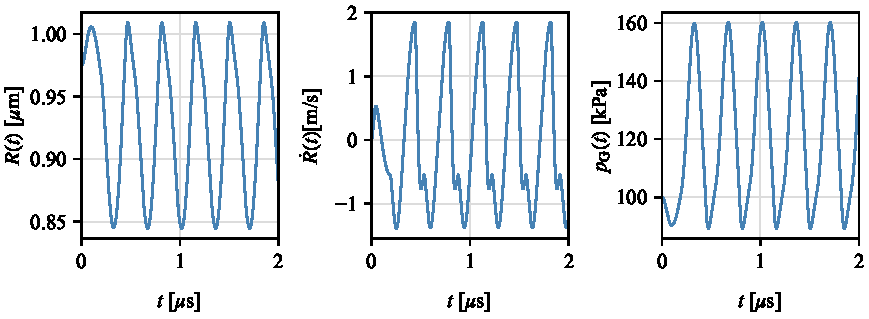
\includegraphics[width=\linewidth]{./figures/ultrasound_lipidcoated_simple.pdf}
    \caption{Temporal evolution of the radius $R(t)$, bubble wall velocity $\dot{R}(t)$ and gas pressure $p_\mathrm{G}(t)$ of a lipid-coated microbubble with initial radius $R_0 = 0.975 \, \upmu \mathrm{m}$, driven by ultrasound with a frequency of $2.9 \, \mathrm{MHz}$ and a pressure amplitude of $130 \, \mathrm{kPa}$, as previously considered by \citet{Marmottant2005}. This example can be found in {\tt \$APECSS\_DIR/examples/ultrasound}, called {\tt lipidcoated\_simple}.}
    \label{fig:bubble_results}
\end{figure}
\chapter{Acoustic emissions}

Modeling the acoustic emissions is a core feature of APECSS. To this end, APECSS offers different models for the acoustic emissions, assuming an incompressible liquid, a weakly-compressible liquid or a fully compressible liquid. To account for a finite propagation speed, the information associated with an emitted acoustic wave is propagated along the radial coordinate axis using a Lagrangian wave tracking approach. Please refer to the work of \citet{Denner2023} for a detailed explanation and validation of the different emission models. Unless specifically told to do so, APECSS does not compute any acoustic emissions. 

\vspace{0.8em}

\noindent
\begin{tabular}{p{0.1\textwidth} p{0.32\textwidth} p{0.5\textwidth}}
    \textbf{Section} &\textbf{Command} & \textbf{Description} 
\vspace{1mm} \\ \hline
{\tt BUBBLE} & {\tt Emissions IC <float>} & Computes the acoustic emissions using the standard incompressible model, Section \ref{sec:emissionsic}.\\ 
& {\tt Emissions FSIC <float>} & Computes the acoustic emissions using the finite-speed incompressible model, Section \ref{sec:emissionsfsic}.\\ 
& {\tt Emissions QA <float>} & Computes the acoustic emissions using the quasi-acoustic model, Section \ref{sec:emissionsqa}.\\ 
& {\tt Emissions EV <float>} & Computes the acoustic emissions based on the Kirkwood-Bethe hypothesis, Section \ref{sec:emissionskb}, with the explicit expression for velocity, see Eq.~\eqref{eq:u_rt}.\\ 
& {\tt Emissions TIV <float>} & Computes the acoustic emissions using the model of \citet{Hickling1963} based on the Kirkwood-Bethe hypothesis, Section \ref{sec:emissionskb}, with the temporally-integrated velocity, see Eq.~\eqref{eq:dudt_rt}.\\ 
& {\tt EmissionIntegration Euler} & Integrates the radial position and, if applicable, the velocity using an Euler scheme.\\
& {\tt EmissionIntegration RK4} & Integrates the radial position and, if applicable, the velocity using a conventional fourth-order Runge-Kutta scheme. This is the default.\\
& {\tt KBIterTolerance <float>} & Tolerance $\eta$ for the evaluation of the pressure using a model based on the Kirkwood-Bethe hypothesis in conjunction with the NASG EoS.\\
& {\tt PruneEmissions <float>} & Prune the emission node if the pressure difference with their neighbors is smaller than the defined tolerance.\\
 \hline
\end{tabular} \vspace{0.2em}

The floating-point value given as the final argument of the {\tt Emissions} command defines the cut-off distance beyond which the emissions are not computed. For the standard incompressible assumption this value has no meaning, but a value is required as a dummy to facilitate the correct reading of the options. In addition to the emissions of a spherical bubble, the emissions computed based on the Kirkwood-Bethe hypothesis can also be used for cylindrical bubbles and planar cavities. The description of the theory below, however, is limited to the spherical case.

\section{Lagrangian wave tracking}

APECSS tracks acoustic emissions using a Lagrangian wave tracking approach \citep{Denner2023}, illustrated in Figure \ref{fig:lagrangiantracking}, in which so-called \textit{emission nodes} are propagated in the radial direction with propagation speed $\mathcal{C}$. Each emission node, represented in APECSS as a structure {\tt struct APECSS\_EmissionNode} and part of a linked list of these structures, holds the current radial coordinate $r(t)$, the flow velocity $u(r,t)$, the pressure $p(r,t$) and, if applicable, the enthalpy $h(r,t)$, as well as the invariants $f(\tau)$ and $g(\tau)$ computed based on the solution of the RP model. The radial position of an emission node at time $t$ is given as
\begin{equation}
    r(t) = R(\tau) + \int_\tau^t \mathcal{C}(r,t) \, \mathrm{d}t, 
    \label{eq:r_t}
\end{equation}
In general, the propagation speed is defined by $\mathcal{C}=c+u$, but the actual value used depends on the chosen model.

\begin{figure}
    \begin{center}
    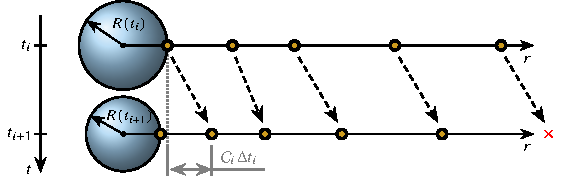
\includegraphics[width=0.7\linewidth]{LagrangianWaveTracking.pdf}
    \caption{Illustration of the Lagrangian transport of the emission nodes, updated at each discrete time instance $t_i$. Nodes that pass a predefined maximum radial coordinate are discarded.}
    \label{fig:lagrangiantracking}
    \end{center}
\end{figure}

\section{Standard incompressible model}
\label{sec:emissionsic}

Assuming an incompressible liquid ($c_{\ell,\mathrm{ref}} \rightarrow  \infty$) with density $\rho_{\ell,\mathrm{ref}}$, the velocity $u(r,t)$ and pressure $p(r,t)$ at a given radial position $r(t)$ are defined as \citep{Neppiras1980}
\begin{equation}
    u(r,t) = \frac{R(t)^2 \dot{R}(t)}{r^2}  \label{eq:u_rt_incomp} 
\end{equation}
and 
\begin{equation}
    p(r,t) = p_\infty(t) + \rho_{\ell,\mathrm{ref}} \left[\frac{R(t)^2 \, \ddot{R}(t) + 2 \, R(t) \, \dot{R}(t)^2}{r} - \frac{R(t)^4 \, \dot{R}(t)^2}{2 \, r^4} \right], \label{eq:p_rt_incomp}
\end{equation}
respectively. The assumption of an incompressible fluid is consistent with the Rayleigh-Plesset models in Eqs.~\eqref{eq:standardRP} and \eqref{eq:modRP}. Note that, because $\mathcal{C} \rightarrow \infty$, these simple incompressible acoustic emissions do not use the Lagrangian wave tracking and no emission nodes are defined and processed, since pressure and velocity are defined instantaneously for all $r$.

\section{Quasi-acoustic model}
\label{sec:emissionsqa}

Assuming the liquid is compressible but accurately described by a constant density $\rho_{\ell,\mathrm{ref}}$ and constant speed of sound $c_{\ell,\mathrm{ref}}$, with $u \ll c_{\ell,\mathrm{ref}}$ and $\mathcal{C} = c_{\ell,\mathrm{ref}}$, \citet{Trilling1952} and \citet{Gilmore1952} derived the {\it quasi-acoustic model} for the acoustic emissions. With the quasi-acoustic model, the velocity, pressure and radial position follow as
\begin{align}
    u(r,t) &= \frac{f(\tau)}{r(t)^2} + \frac{g(\tau)}{r(t) \, c_{\ell,\mathrm{ref}}}  \label{eq:u_rt_qa} \\
  p(r,t) &=  p_\infty(t) + \rho_{\ell,\mathrm{ref}} \left[ \frac{g(\tau)}{r(t)} - \frac{u(r,t)^2}{2} \right] \label{eq:p_rt_qa} \\
  r(t) &\approx R(\tau) + c_{\ell,\mathrm{ref}} \sum_{i=1}^N \Delta t_{i-1}, \label{eq:r_t_qa}
\end{align}
where $f(\tau)$ and $g(\tau)$ are invariants defined based on the result of the employed RP model as
\begin{align}
    f(\tau) &= R(\tau)^2 \dot{R}(\tau) - \frac{R(\tau) g(\tau)}{c_{\ell,\mathrm{ref}}}\\
    g(\tau) &= R(\tau) \left[\frac{p_\mathrm{L}(\tau)-p_\infty(\tau)}{\rho_{\ell,\mathrm{ref}}} + \frac{\dot{R}(\tau)^2}{2} \right], \label{eq:g_qa}
\end{align}
and $\tau$ is the time at which the acoustic information is emitted at the bubble wall. For $t=\tau$ with $r(t)=R(\tau)$, Eq.~(\ref{eq:u_rt_qa}) reduces to $u(R,\tau)=\dot{R}(\tau)$ and Eq.~(\ref{eq:p_rt_qa}) reduces to $p(R,\tau)=p_\mathrm{L}(\tau)$, thus satisfying the boundary conditions at the bubble wall. 

The quasi-acoustic model is consistent in its modelling assumptions with the Keller-Miksis model, Eq.~\eqref{eq:keller}. The applicability of the quasi-acoustic model is limited to small Mach numbers, $(\dot{R}/c_0)^2 \ll 1$, as it incorporates a finite propagation speed of the acoustic emissions and the nonlinear pressure contributions resulting from the flow, but since all parts of the wave propagate with speed $c_0$, the quasi-acoustic model can neither describe the nonlinear distortion of acoustic waves nor the formation of shock fronts. 

\section{Finite-speed incompressible model}
\label{sec:emissionsfsic}

APECSS also supports the assumption that the liquid is incompressible but the information associated with the acoustic emissions still propagates with finite speed $\mathcal{C} = c_{\ell,\mathrm{ref}}$ using the Lagrangian wave tracking approach, with the radial location given by Eq.~\eqref{eq:r_t_qa}.
By assuming the specific acoustic impedance of an incompressible liquid, $\rho_{\ell,\mathrm{ref}} c_{\ell,\mathrm{ref}} \rightarrow \infty$, the velocity reduces to
\begin{align}
    u(r,t) = \frac{R(\tau)^2 \dot{R}(\tau)}{r(t)^2}, \label{eq:u_rt_fsic} 
\end{align}
while $p(r,t)$ and $g(\tau)$ are given by Eq.~\eqref{eq:p_rt_qa} and Eq.~\eqref{eq:g_qa}, respectively.
This approach, referred to in APECSS as {\tt FSIC} or \text{finite-speed incompressible model}, recovers the time delay between emitting information at the bubble wall and this information arriving in a certain location, but treats the flow field as incompressible.

\section{Emissions based on the Kirkwood-Bethe hypothesis}
\label{sec:emissionskb}

Under the Kirkwood-Bethe hypothesis \citep{Kirkwood1942,Cole1948}, the propagation speed along the outgoing characteristic is given as $\mathcal{C}(r,t) = c(r,t) + u(r,t)$. The ODE describing the radial position along the outgoing characteristics is, thus, defined as 
\begin{equation}
    \left. \frac{\mathrm{d}r(t)}{\mathrm{d}t} \right|_\text{c} = c(r,t) + u(r,t). \label{eq:drdt}
\end{equation}
This ODE is numerically integrated using either an Euler scheme or a fourth-order Runge-Kutta (RK4) scheme, with initial condition $r(t) = R(\tau)$ for $t=\tau$, where $\tau$ is the time at which the acoustic information is emitted at the bubble wall. The time step $\Delta t$ is taken to be the same as used for the integration of the model describing the bubble dynamics (see Section \ref{chap:bubble}).

Two models to compute the velocity $u(r,t)$ at a given emission node are available in APECSS: (i) an explicit expression for $u(r,t)$ \citep{Denner2023}  and (ii) integrating the temporal derivative of the velocity, $\mathrm{d}u(r,t)/\mathrm{d}t$, along the outgoing characteristic, as proposed by \citet{Hickling1963}. The assumptions used to derive these models for the acoustic emissions are consistent with the Gilmore model, Eq.~\eqref{eq:gilmore}.

Following a similar derivation as for the quasi-acoustic model discussed in Section \ref{sec:emissionsqa}, but assuming a fully-compressible liquid described by a suitable equation of state, the {\it explicit velocity (EV)} is given as
\begin{equation}
    u(r,t) = \frac{f(\tau)}{r(t)^2} + \frac{g(\tau)}{r(t) \, [c(r,t) + u(r,t)]} , \label{eq:u_rt}
\end{equation}
with 
\begin{equation}
    f(\tau) = R(\tau)^2 \dot{R}(\tau) - \frac{R(\tau) \, g(\tau)}{c_\mathrm{L}(\tau) + \dot{R}(\tau)}  . \label{eq:f_R}
\end{equation}
For $t=\tau$ with $r(t)=R(\tau)$, this expression reduces to $u(R,\tau)=\dot{R}(\tau)$, thus satisfying the boundary conditions at the bubble wall.

\citet{Hickling1963} proposed to integrate the velocity with respect to time, in APECSS referred to as {\it temporally-integrated velocity (TIV)}, with the temporal derivative of the velocity along the outgoing characteristic given as
\begin{equation}
    \left. \frac{\mathrm{d}u(r,t)}{\mathrm{d}t} \right|_\text{c} =  - \frac{2 c(r,t)^2 u(r,t)}{r(t) \, [c(r,t)-u(r,t)]} + \frac{g(\tau)}{r(t)^2} \, \frac{c(r,t)+u(r,t)}{c(r,t)-u(r,t)}. \label{eq:dudt_rt}
\end{equation}
This differential equation for the velocity is integrated together with the equation for ${\mathrm{d}r(t)/\mathrm{d}t}$, Eq.~\eqref{eq:drdt}, using the initial condition $u(R,\tau) = \dot{R}(\tau)$. 

Regardless of the choice of velocity model, the invariant $g(\tau)$ is defined as
\begin{align}
    g(\tau) = R(\tau) \left[h_\mathrm{L}(\tau) - h_\infty(\tau) + \frac{\dot{R}(\tau)^2}{2} \right]
    \label{eq:g_R} .
\end{align}
For a given radial position $r(t)$ and flow velocity $u(r,t)$, irrespective of which model is used to compute the velocity, the enthalpy is readily evaluated as
\begin{equation}
    h(r,t) = h_\infty(t) + \frac{g(\tau)}{r(t)} - \frac{u(r,t)^2}{2}, \label{eq:h_rt}
\end{equation}
where $h_\infty$ is spatially invariant and only depends on time. For $t=\tau$ with $r(t)=R(\tau)$, this expression for enthalpy reduces to $h(R,\tau)=h_\mathrm{L}(\tau)$, satisfying the boundary conditions at the bubble wall. 

Using the Tait EoS, the pressure can be readily computed from the enthalpy defined in Eq.~(\ref{eq:h_rt}) by inserting Eq.~(\ref{eq:rho_Tait}) into Eq.~(\ref{eq:h_Tait}) and rearranging to yield
\begin{equation}
    p(r,t) = \left[ \frac{(\Gamma-1) \, \rho_0}{\Gamma \, (p_0+B)^{1/\Gamma}} \, h(r,t) \right]^{\frac{1}{1-1/\Gamma}} - B. \label{eq:p_rt}
\end{equation}
Solving Eq.~(\ref{eq:p_rt}) is straightforward because the enthalpy $h(r,t)$ is the only variable, all other quantities are predefined fluid properties. Using the NASG EoS, pressure $p(r,t)$ follows by rearranging Eq.~(\ref{eq:h_NASG}) as
\begin{eqnarray}
p(r,t) = \frac{\left[\Gamma-1\right] \rho(r,t) \, h(r,t) - \left[1 - b \, \rho(r,t) \right] \Gamma B}{\Gamma - b \, \rho(r,t)}.  \label{eq:p_rt_NASG}
\end{eqnarray}
Since the pressure $p(r,t)$ and the density $\rho(r,t)$ depend explicitly on each other in this formulation, Eq.~(\ref{eq:p_rt_NASG}) has to be solved iteratively. As a convergence criterion for the iterative approximation we use $|p_j(r,t) - p_{j-1}(r,t)| < \eta \, |p_j(r,t)|$, where $j$ denotes the iteration counter and $\eta$ is a predefined tolerance (see option {\tt KBIterTolerance}). Preliminary tests identified a tolerance of $\eta = 10^{-4}$ to be sufficiently small.

Emission nodes with a higher pressure propagate faster than nodes with a lower pressure, which in turn leads to progressive steepening of the acoustic wave. As a result, an emission node may overtake the forerunning emission node, yielding an unphysical multivalued solution. In reality, such a multivalued solution is avoided by the formation of a shock front \citep{Fay1931}. While treating such multivalued solutions is often done in a post-processing step, APECSS deals with multivalued solutions at run time. An emission node that overtakes its forerunning neighbor is discarded, see Fig.~\ref{fig:lagrangiantrackingshock}, and the thermodynamic values of the forerunning neighbor are reevaluated by a simple averaging procedure. Thus, a unique and physically plausible solution is maintained.

\begin{figure}
    \begin{center}
    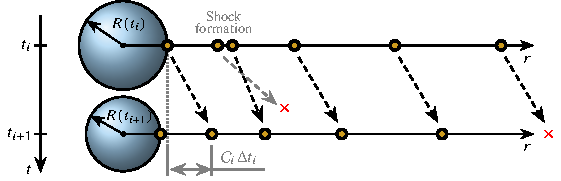
\includegraphics[width=0.7\linewidth]{LagrangianWaveTracking_withShock.pdf}
    \caption{Illustration of the Lagrangian transport of the emission nodes, updated at each discrete time instance $t_i$. Nodes that either overtake the forerunning node, which represents the formation of a shock front, or that pass a predefined maximum radial coordinate are discarded.}
    \label{fig:lagrangiantrackingshock}
    \end{center}
\end{figure}


\section{Results}
\label{sec:emissions_results}

APECSS can write out different results based on the acoustic emissions. Note that APECSS does \uline{not} write any results to disk unless it is specifically ask to do so.

The acoustic emissions can be recorded as a function of time at one or multiple radial locations (cf.~{\tt EmissionsSpace}), or the emissions are written out with respect to their radial location at one or multiple time instances (cf.~{\tt EmissionsTime}) or emission nodes (cf.~{\tt EmissionsNode}), or for selected extrema in a specified period (cf.~{\tt EmissionsMinMax}). This calls can be used multiple times to defined, for instance, multiple radial locations or time instances.

\vspace{0.8em}

\noindent
\begin{tabular}{p{0.1\textwidth} p{0.36\textwidth} p{0.49\textwidth}}
    \textbf{Section} &\textbf{Command} & \textbf{Description} 
\vspace{1mm} \\ \hline
{\tt RESULTS} & {\tt OutputPath <string>} & Path to the folder where all the results should be written in to (default: {\tt ./}).\\
& {\tt OutputDigits <int>} & Results are written out with as many digits (default: 6).\\
& {\tt EmissionsSpace <float>} & Defines a radial location at which the emissions in the liquid are written out as a function of time. If/while the location is in the gas phase, $0$ is recorded.\\ 
& {\tt OutputFreqEmissionsSpace <int>} & Results of the emissions at a specific radial location are stored every so many time steps (default: 1).\\ 
& {\tt EmissionsTime <float>} & Defines a time instance at which the emission in the liquid are written out as a function of the radial coordinate.\\ 
& {\tt EmissionsNode <int>} & Defines a node ID of which the emission in the liquid are written out as a function of the radial coordinate.\\ 
& {\tt EmissionsMinMax <int>} & Defines the period in which the emission in the liquid are written out as a function of the radial coordinate for the node representing $R_\mathrm{min}$, $\dot{R}_\mathrm{min}$ and $p_\mathrm{L,max}$.\\ 
 \hline
\end{tabular}

The first line of the results file(s) lists the variables that were written out and their order. For instance, Figure \ref{fig:emissions_results} shows the different ways in which emissions can be recorded, using the sonoluminescence example found in the {\tt \$APECSS\_DIR/examples/ultrasound/} folder.

\begin{figure}
    \centering
    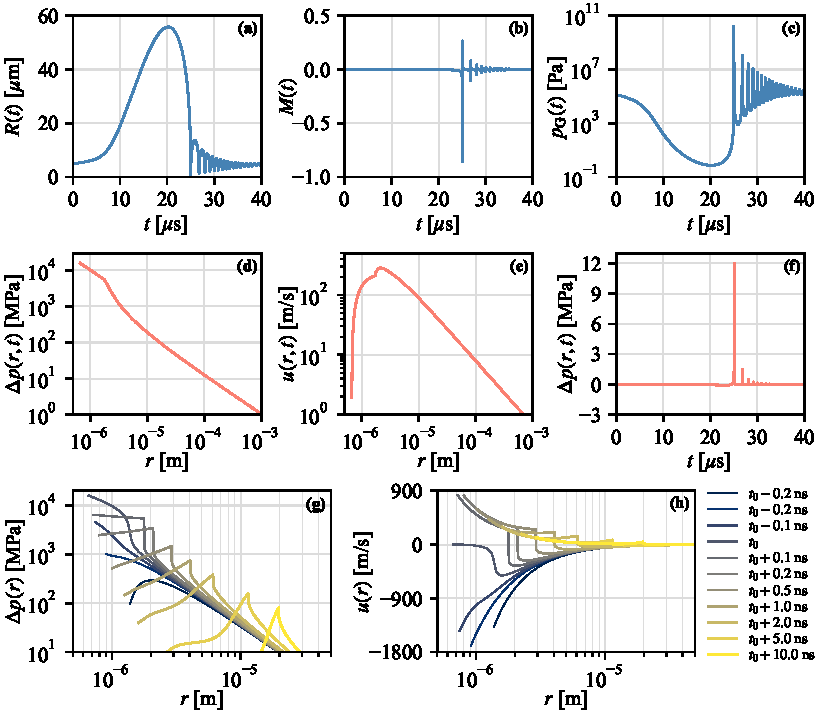
\includegraphics[width=\linewidth]{./figures/emissions_results.pdf}
    \caption{Results of an argon bubble with initial radius $R_0 = 5 \, \upmu \mathrm{m}$ in water, driven by ultrasound with a frequency of $23.5 \, \mathrm{kHz}$ and a pressure amplitude of $145 \, \mathrm{kPa}$, as previously considered by \citet{Holzfuss2010}. {\bf(a)}-{\bf(c)} The bubble radius $R(t)$, bubble-wall Mach number $M(t)=\dot{R}(t)/c_\mathrm{L}(t)$, and gas pressure $p_\mathrm{G}(t)$ as a function of time $t$. {\bf(d)}-{\bf(e)} The pressure amplitude $\Updelta p(r,t)$ and velocity $u(r,t)$  of the acoustic wave generated by the primary collapse of the bubble as a function of the radial coordinate $r$. {\bf (f)} The pressure amplitude $\Updelta p(r,t)$ emitted by the bubble at a fixed radial distance $r=100 \, \upmu \mathrm{m}$ from the bubble center as a function of time $t$. {\bf(g)}-{\bf(h)} Spatial profiles of the pressure amplitude $\Delta p(r,t)$ and the velocity $u(r,t)$ at selected time instances, where $t_0$ is the time at which the bubble assumes its minimum radius. This example can be found in {\tt \$APECSS\_DIR/examples/ultrasound}, called {\tt sonolum\_emissions}.}
    \label{fig:emissions_results}
\end{figure}

\cleardoublepage

\addcontentsline{toc}{chapter}{Bibliography}
\bibliographystyle{natbib}
\bibliography{/Users/fabian/Zotero/library}
\end{document}